\section{Auswertung}
\subsection{Versuchsaufbau}

\subsection{Kalibrierung}
Zunächst haben wir manuell eine Hallsonde in etwa im Zentrum des
Magnetspulenpaars positioniert, was dadurch erreicht wurde, dass die Position
der Sonde so lange verändert wurde, bis der maximale Wert des digital
ausgegebenen Messwerts der Hallsonde erreicht war. Da dann die Mitte des
Spulenpaars gefunden war, wurde die Hallsonde selbst im weiteren Experiment
nicht mehr bewegt. Die Messunsicherheit der Magnetfeldmessung liegt immer bei
der letzten angegebenen Nachkommastelle, also ist dieser Fehler hier $\pm
\SI{1}{\milli\tesla}$.

Da wir nun eine Möglichkeit hatten, Magnetfelder zu messen, wurde als Nächstes
das bei verschiedenen Stromstärken resultierende Magnetfeld untersucht. Dafür
wurde das Magnetfeld in \SI{1}{\ampere}"~Schritten von \SI{0}{\ampere} bis etwa
\SI{10,8}{\ampere} bzw.
\SI{-10,8}{\ampere} verändert und das jeweils
zugehörige Magnetfeld wurde als Messwert aufgenommen. Um den Einfluss von
Hysterese-Effekten zu untersuchen, wurde immer von kleinen zu großen
Stromstärken $I$ und anschließend wieder zurück von großen zu kleinen
Stromstärken gemessen. Dieses Vorgehen eignet sich, um die Größe der
Restmagnetisierung bei $I=0$ zu bestimmen. Die Messwerte können im Anhang
\ref{sec:messwerte} betrachtet werden. 

Wenn man nun diese Datenpunkte in einem Diagramm aufträgt, resultiert das in
\fref{hysterese} dargestellte Bild.

\begin{figure}[htb]
   \centering
   \includegraphics[width=1\columnwidth,keepaspectratio]{../tmp/hysteresis}
   \caption{Magnetfeldstärke in Abhängigkeit vom Erregerstrom $I$}
   \label{fig:hysterese}
\end{figure}

Wie man erkennen kann, ist nicht nur eine durchgehende Linie sichtbar, sondern
eine klassische Hysteresekurve mit zwei einzelnen Linien jeweils für $I<0$ und
für $I>0$ ist erkennbar. Allerdings verzichten wir im Weiteren auf eine genaue
Untersuchung der eingeschlossenen Fläche, sondern betrachten die Kurve als
jeweils eine Linie, und der Einfluss der Hysterese wird als Fehler dieser
Annahme betrachtet. Dies ist legitim, da die Abstände der Linien nie mehr als
ca. \SI{10}{\milli\tesla} beträgt, während die Messwerte schnell Bereiche von
100 bis \SI{500}{\milli\tesla} erreichen, sodass der Fehler dabei im
Prozentbereich liegt.

\subsection{Messung des elektrischen Widerstands des Kristalls bei
Raumtemperatur}
Um eine Vorstellung der Größenordnung der Widerstände, die zwischen den
einzelnen Kontakten unseres Halbleiterkristalls bestehen, zu erhalten, wurden
verschiedene Kombinationen von Kontakten daraufhin vermessen. Dabei haben wir
festgestellt, dass bei unserer Probe der Kontakt mit der Nummer fünf defekt
ist, sodass nur die anderen im weiteren Versuch verwendet werden konnten. Die
einzelnen Messergebnisse der Widerstandsmessung können im Anhang
\ref{sec:messwerte} betrachtet werden. Wie man erkennen kann, liegen die
Werte, bei denen beide Messpunkte zum gleichen Kontakt gehörten, während die
eine Messspitze direkt an der Probe und die andere am Messpad anlag, im Bereich
um \SI{1}{\ohm}. Dies ist demnach die Größenordnung der Kabelwiderstände
inklusive der Kontaktwiderstände. Wenn nun der Widerstand zwischen
unterschiedlichen Kontaktpunkten gemessen wird, kann man feststellen, dass die 
Werte in einer ganz anderen Größenordnung von etwa 20 bis \SI{50}{\ohm} liegen.
Die Werte für die realen Widerstände liegen also im eben angegebenen Bereich,
wobei der Fehler durch die vorher beschriebenen Kontakt- und Kabelwiderstände
vernachlässigt werden kann, da diese wesentlich kleiner sind. Es muss aber
erwähnt werden, dass dieses Ergebnis nur bei Zimmertemperatur gültig ist, da
sich der Widerstand stark mit der Temperatur ändern wird.

\subsection{Messverfahren}

Die automatisch Messapparatur misst pro Temperatur $T$ insgesamt sechs Spannung.
Jene werden im \cite{script} näher erläutert. Man stellt fest, dass die
Spanunng $U_H$ sowie auch $U_ρ$, deren Bedeutung noch erläutert wird, zweimal
gemessen werden. Dies geschieht für beide möglichen, senkrechten Orientierungen
des Magnetfeldes und wird durch eine Umkehrung des Spulenstroms $I$ erreicht.
Bei der Umkehrung des Magnetfeldes kehren sich auch die beiden gemessenen Spannungen
um, nicht jedoch aber die systematischen Verschiebungen, wie zum Beispiel der
Thermospannung wegen ungleichmäßiger Kühlung oder etwaige Spannungsdifferenzen
auf Grund der Geometrie der Halbleiterprobe.
\begin{equation}
 U_{\mbox{mess.}}^± = ± U + U_{\mbox{syst.}}
\end{equation}
Durch das zweimalige Messen der Spannungen bei verschieden orientiertem Magnetfeld lässt sich schließlich eine Spannung
$U$ errechnen, die frei von diesen systematischen Fehlern ist.
\begin{equation}
 U = \frac{U_{\mbox{mess.}}^+ - U_{\mbox{mess.}}^-}{2}
\end{equation}
Dieses Prinzip wurde für alle aus den Messdaten entnommenen Spannungen angewendet.



\subsection{Messung des temperaturabhängigen spezifischen Widerstands}

\begin{figure}[htb]
   \centering
   \includegraphics[width=1\columnwidth,keepaspectratio]{../tmp/temperatur}
   \caption{Temperatur $T$ in K in Abhängigkeit der Zeit}
   \label{fig:temp}
\end{figure}

Als erstes wurde nun bei eingeschaltetem Kryostaten, der die Temperatur
kontinuierlich von anfänglich Zimmertemperatur auf schließlich ca.
\SI{54,3}{\kelvin} absenkte und anschließend wieder auf Raumtemperatur
aufheizte. Jegliche Messung, die während dieser Phase durchgeführt wurde, wurde
mittels eines computergestützten Steuerungsprogramm ausgeführt. Damit dieses
die Messgeräte korrekt ansteuern konnte, musste die dem \cite{script} entnommene
\fref{Schaltung} aufgebaut werden.

\begin{figure}[htb]
 \centering
 \includegraphics[page=6,viewport=70 395 525 705,clip,width=\columnwidth,keepaspectratio]{../docs/Anleitung_Hall.pdf}
 \caption{Schaltung zur rechnergesteuerten Datennahme}
 \label{fig:Schaltung}
\end{figure}

Um aus den aufgenommenen Messwerten den spezifischen Widerstand berechnen zu
können, wird eine Umrechnungsformel benötigt. Der spezifische Widerstand ρ ist
nach \cite[Gl. (12.30)]{ibach}wie folgt definiert:
\begin{equation}
ρ = R\frac{A}{l} = \frac{A}{I\cdot l} U_ρ
\label{eqn:rho}
\end{equation}
Hierbei ist $U_ρ$ der gemessene Spannungsabfall über den Kontakten 3 und 4 der Probe,
$A= b\cdot d$ der Querschnitt des Kristalls, und $l$ der Abstand zwischen den
beiden Spannungsmesspunkten an der Probe. Die Probeneigenschaften $b, d, l$ können
der \tref{daten} im Anhang unter Proben-Nr. 2 entnommen werden.
Der maximale Strom ist mit
\begin{equation}
 I = \SI{1,0}{\milli\ampere} 
\end{equation}
angegeben, und dieser Wert wurde auch von der Messapparatur automatisch nachgeregelt.
Somit kann also über die Messung von $U_ρ(T)$ und \eref{rho} der spezifische Widerstand in
Abhängigkeit von der Temperatur angegeben werden. Das schließlich resultierende
Diagramm ist in \fref{spezWS} dargestellt.

\begin{figure}[htb]
   \centering
   \includegraphics[width=1\columnwidth,keepaspectratio]{../tmp/spezWS}
   \caption{spezifischer Widerstand in Abhängigkeit von der inversen Temperatur}
   \label{fig:spezWS}
\end{figure}

% Die Einheit von ρ ist hierbei \SI{1}{\ohm\meter}.
Wie man erkennen kann, existiert ein Maximum des spezifischen Widerstands.
Außerdem ist ersichtlich, dass sich $ρ$ für kleine $T$, also große $T^{-1}$,
weniger stark ändert, als für große $T$.
Der Graph von ρ lässt sich in zwei
näherungsweise lineare Abschnitte einteilen. Für kleine $T^{-1}$ ist wächst ρ
exponentiell, um schließlich für große $T^{-1}$ exponentiell schwach zu fallen.
% Bei Raumtemperatur und bei der minimalen Temperatur von ca. \SI{54}{\kelvin} sind
% die Widerstände wieder ähnlich groß.

Es sind hierbei pro Temperaturwert $T$ jeweils zwei Werte für ρ angegeben, da $U_ρ(T)$
einmal beim Abkühlen und dann nochmal beim Aufwärmen für $T$ gemessen werden konnte.
Dies lässt sich auch gut in \fref{temp} erkennen.

In diesem wie auch in den folgenden Diagrammen waren nun die Gebiete der
Störstellenleitung sowie der Eigenleitung zu identifizieren. Bei der
Störstellenleitung handelt es sich um eine elektrische Leitfähigkeit, die durch
die Dotierung des Halbleitermaterials zustande kommt. Bei der Dotierung werden
Fremdatome in das Gitter, das ganz regelmäßig aus gleichartigen Atomen bzw.
Molekülen aufgebaut ist, eingebracht. Diese Fremdatome stellen zusätzliche
Ladungsträger bereit. Wenn diese Störstellenatome mehr Valenzelektronen besitzen
als die umgebenden Atome, so sind diese Elektronen als quasifrei anzusehen.
Daher werden solche Fremdatome in diesem Fall als Donatoren bezeichnet, da sie
zusätzliche Elektronen bereitstellen. Wenn sie allerdings über weniger
Valenzelektronen als die Umgebung verfügen, so handelt es sich um Löcher als
zusätzliche Ladungsträger.

Die Störstellenleitung, die auf der Existenz dieser Fremdatome beruht, tritt
bereits bei kleinen Temperaturen auf, da die eben genannten Ladungsträger
quasifrei sind und somit geringe elektrische Spannungen ausreichen, um dafür zu
sorgen, dass sie sich durch des Kristall bewegen, also einen Stromfluss
darstellen.

Bei der Eigenleitung, die auch bei undotierten Halbleitermaterialien auftritt,
werden hingegen große Temperaturen benötigt, da erst die hohe thermische Energie
dafür sorgt, dass die Ladungsträger, die sich nahe der Fermienergie befinden, im
Leitungsband aufhalten können und somit eine endliche Leitfähigkeit hergestellt
werden kann. 

Im dargestellten Diagramm in \fref{spezWS} ist also der Bereich bei kleinen
inversen Temperaturen (also bei großen Temperaturen) auf die Eigenleitung
kombiniert mit der Störstellenleitung zurückzuführen, während bei kleinen
Temperaturen (großen inversen Temperaturen) ausschließlich Störstellenleitung
auftritt. Man kann der Abb. also entnehmen, dass für kleine Temperaturen,
bei dem es nur Störstellenleitung und keine Eigenleitung gibt, der spezifische
Widerstand hoch ist und für steigende Temperaturen zunächst leicht zunimmt, um
dann schließlich bei ungefähr bei $T^{-1} = \SI{0,009}{\per\kelvin}$ also bei \SI{111}{\kelvin}
abzufallen. Bei sehr kleinen Temperaturen (kleiner als die hier verwendeten)
sollte der spezifische Widerstand sinken, da in diesem Störstellenreserve
genannten Temperaturbereich nach und nach immer mehr der Ladungen
der vorhandenen Fremdatome durch die immer höhere thermische Energie ihre
Bindung zum Atomrumpf verlieren. Somit stehen also immer mehr quasifreie
Ladungsträger zur Verfügung, was sich im Absinken des Widerstands bemerkbar
machen sollte. Im darauf folgenden Bereich, der hier auch dargestellt ist bei
kleinen Temperaturen, der Störstellenerschöpfung, steigt der spezifische
Widerstand bei steigender Temperatur an, weil hier keine neuen Ladungsträger
der Fremdatome hinzukommen, dafür aber wie bei Metallen durch die steigende
Temperatur die Ladungen am ungehinderten Fließen gehindert werden. Somit steigt
hier der Widerstand an. Ein weiterer Effekt bewirkt das Ansteigen des
Widerstands: Wie man an \fref{hallkonstante2} erkennen kann, wechselt die
Hallkonstante bei der Übergangstemperatur ihr Vorzeichen, was bedeutet, dass
die Majoritätsladungsträger wechseln. Bis zu diesem Wert nimmt also die
effektive Ladungsträgerdichte ab, was sich ebenfalls im Ansteigen des
Widerstands manifestiert. Bei weiter ansteigender Temperatur tritt nun die in
einem fließenden Übergang die Eigenleitung verstärkt auf, wie sie oben bereits
beschrieben wurde. Da hier immer mehr Ladungsträger zur Verfügung stehen, kann
der spezifische Widerstand mit steigender Temperatur absinken.

Anhand dieser Grafik kann man jedoch noch nicht besonders gut die Grenze
zwischen den beiden Leitungstypen erkennen. Eine genauere
Untersuchung wird bei den folgenden Diagrammen durchgeführt.

\subsection{Messung der temperaturabhängigen Hallkonstante}

Weiterhin war die Temperaturabhängigkeit der Hall-Konstante unseres Materials
$R_H$ zu untersuchen. Gemäß \cite[Gl. (XIV.2)]{ibach} kann die Hall-Konstante
wie folgt berechnet werden: 
\begin{equation}
R_H = \frac{d}{I B} U_H
\end{equation}
Es kann also wieder über die Messung der Temperaturabhängigkeit einer Spannung
(hier der Hallspannung $U_H$) die Temperaturabhängigkeit der uns
interessierenden Messgröße (hier die Hall-Konstante) bestimmt werden. Bei
diesen Messungen betrug der Magnetspulenstrom \SI{8}{\ampere}, was einer
magnetischen Flussdichte von
\begin{equation}
 B=\SI{443(4)}{\milli\tesla}
\end{equation}
entspricht.
Da alle Größen bekannt sind, kann nun das Diagramm in \fref{hallkonstante}
erstellt werden, in dem die Temperaturabhängigkeit der Hallkonstante dargestellt ist.
\begin{figure}[htb]
   \centering
   \includegraphics[width=1\columnwidth,keepaspectratio]{../tmp/hallkonstante}
   \caption{Logarithmus der Hallkonstante $R_H$ in Abhängigkeit von der inversen Temperatur $T^{-1}$}
   \label{fig:hallkonstante}
\end{figure}

Die Hallkonstante ist in gewisser Weise ein Maß für die
Ladungsträgerkonzentrationen $n$ und $p$, was man an der folgenden, \cite[Gl.
XIV.5]{ibach} entnommenen Gleichung erkennen kann:
\begin{equation}
R_H = \frac{pμ_p^2-nμ_n^2}{e(pμ_p+nμ_n)^2}
\end{equation}
Diese Gleichung ist für beide Leitungstypen gültig. Im Falle der
Störstellenleitung ist aber, abhängig davon, ob es sich bei den Störstellen um
Akzeptoren oder Donatoren handelt, eine der Konzentrationen gleich null, sodass
sich diese Gleichung zu der folgenden vereinfacht:
\begin{equation}
\label{eqn:hallkonst}
R_H = -\frac{1}{ne}
\end{equation}
Hierbei ist $e$ die Elementarladung. Das Vorzeichen der Hallkonstante sagt
somit aus, um welchen Leitungstypen es sich bei den gegebenen Umständen wie
der Temperatur handelt. Ein negatives Vorzeichen bedeutet, dass es sich
hauptsächlich um Elektronen als Ladungsträger handelt, dass also ein
n-Halbleiter vorliegt.

Die hier auftauchenden Ladungsträgerkonzentrationen können auch negativ sein.
Dies bedeutet, dass pro Volumeneinheit weniger als null dieser Ladungsträger
vorhanden sind, was sich so erklären lässt, dass sich in diesem Raumgebiet mehr
von den anderen Ladungsträgern befinden als von den durch die Konzentration
angegebenen.

Auch hier teilt sich die Kurve in die drei oben genannten Bereiche auf, nur
dass man hier genauer den Bereich des Übergangs von der Störstellenleitung zur
Eigenleitung erkennen kann. Diesen Bereich kann man hier mit etwa $0,007\le 1/T
\le 0,009$ angeben. In \tref{bereiche} sind die Einordnungen noch einmal
übersichtlich zusammengestellt.

\begin{table}[htbp]
\centering
\setlength{\tabcolsep}{2.5pt}
\begin{tabular*}{0.95\columnwidth}{%
S[tabformat=1.3]%
S[tabformat=1.2]%
}
\toprule
{Leitungsbereich} & {inv. Temp. T$^{-1}$ in [K$^{-1}$]}\\
\midrule
{Störstellenleitung} & {T$^{-1} > 0,009$}\\
{Übergangsbereich} & {$0,007 \le$ T$^{-1} \le 0,009$}\\
{Eigenleitung} & {T$^{-1} < 0,007$}\\
\bottomrule
\end{tabular*}
\caption{Zuordnung der Leitungsbereiche zu den Bereichen der inversen
Temperatur}
\label{tab:bereiche}
\end{table}

\begin{figure}[htb]
   \centering
   \includegraphics[width=1\columnwidth,keepaspectratio]{../tmp/hallkonstante2}
   \caption{Hallkonstante $R_H$ in Abhängigkeit von der inversen Temperatur $T^{-1}$}
   \label{fig:hallkonstante2}
\end{figure}

In der Grafik erkennt man den Vorzeichenwechsel am starken Absinken bei
ungefähr $1/T \approx \SI{0.008}{\per\kelvin}$ \^{=} \SI{125}{\kelvin}, da in
diesem Bereich kleine Werte der Hallkonstante vorliegen und somit der
Logarithmus gegen $-\infty$ geht, was aufgrund der nicht exakt null werdenden
Hallkonstante nicht der Fall ist, aber dennoch wird hier deutlich das globale
Minimum eingenommen. Der Vorzeichenwechsel ist ebenso auch in der nicht logarithmischen
\fref{hallkonstante2} zu erkennen.

Aus der Tatsache, dass es sich um einen Vorzeichenwechsel handelt,
kann man gemäß \eref{hallkonst} schließen, dass es einen
Übergang gibt, bei dem der eine Ladungsträgertyp allmählich durch den anderen
als dominanter Ladungsträger abgelöst wird. In unserem Fall hat die
Hallkonstante bei kleinen Temperaturen ein positives Vorzeichen, woraus
ersichtlich wird, dass es sich bei diesen Temperaturen hauptsächlich um Löcher
handelt, die die Ladungen transportieren. Daraus kann man nun ableiten, dass es
sich bei unserer Probe um einen p-dotierten Halbleiter handelt. Bei größeren
Temperaturen aber kehrt sich das Vorzeichen um und es sind vor allem Elektronen,
die bei diesen Temperaturen die Ladungen transportieren.

\subsection{Weitere elektronische Eigenschaften der Probe}

Schließlich sollte ein weiteres Diagramm angefertigt werden, in dem
$\ln\{R_H(T/300)^{3/2}\}$ als Funktion von $1/T$ dargestellt ist. Dieses
Diagramm ist in \fref{funktion} dargestellt.

\begin{figure}[htb]
   \centering
   \includegraphics[width=1\columnwidth,keepaspectratio]{../tmp/funktion}
   \caption{$\ln\{R_H(T/300)^{3/2}\}$ in Abhängigkeit von der inversen
   Temperatur}
   \label{fig:funktion}
\end{figure}

Wie man sehen kann, ähnelt dieses Diagramm stark demjenigen, das in
\fref{hallkonstante} dargestellt ist. Einzig bei sehr kleinen Temperaturen,
also großen inversen Temperaturen, fällt in diesem Diagramm der Ast etwas
stärker ab als im vorigen Diagramm.

\subsection{Messung der Ladungsträgerkonzentrationen}

Im folgenden soll nun die Ladungsträgerkonzentrationen $n$ bei einer Temperatur von
$T = \SI{77}{\kelvin}$ bestimmt werden. Hierfür gehen wir von \eref{hallkonst}
aus
und erhalten:
\begin{equation}
 n = -\frac{1}{R_H e}
\end{equation}
Die Hallkonstante für die entsprechende Temperatur lässt sich der
\fref{hallkonstante2} entnehmen. Bei Mittelung über beide Werte der Konstante
erhält man:
\begin{equation*}
 R_H(\SI{77}{\kelvin}) = \SI{1,79(1)e-3}{\meter\cubed\per\coulomb}
\end{equation*}
Setzt man dies nun in obige Gleichung ein, so lässt sich $n$ berechnen.
\begin{equation*}
 n = \SI{-3,49(2)e21}{\per\meter\cubed}
\end{equation*}
Um eine Vorstellung davon zu bekommen, was dies bedeutet, führen wir hier eine
kleine Vergleichsrechnung durch. Wenn man eine Dichte unseres Materials von
\SI{5}{\gram\centi\meter\tothe{-3}} und eine molare Masse von Tellur annimmt,
so befinden sich in einem Kubikmeter etwa $3\cdot 10^{28}$ Atome, woran man
erkennen kann, dass nur ca. ein Atom auf $10^7$ ionisiert wird. Im Vergleich
dazu gibt beim Kupfer jedes Atom mehr als ein Elektron ab, was die viel bessere
Leitfähigkeit von Metallen noch einmal verdeutlicht.

\subsection{Messung der Bandlücke}

Bei hohen Temperaturen überwiegt im Halbleiter die Eigenleitung gegenüber der
Störstellenleitung. Dieser Bereich ist bei uns durch die abfallende, linke Flanke
in \fref{hallkonstante} gegeben. Gehen wir also im folgenden davon aus, dass
die Eigenleitung ab $\frac{1}{T} = \SI{0.0065}{\per\kelvin}$ überwiegt, was wiederum
ungefähr $\SI{154}{\kelvin}$ entspricht. In diesem Bereich gilt für die
Ladungsträgerdichte
\begin{equation}
 n = \mbox{const.} \, \cdot T^{3/2}\cdot e^{\frac{-1}{2k_BT}}
 \label{eqn:n_T}
\end{equation}
. Für die Leitfähigkeit σ gilt $σ = \frac{1}{ρ} = nμe$, woraus sich eine
Abhängigkeit zwischen ρ und $n$ ergibt. Weiterhin wird angenommen, dass die
Beweglichkeit μ für hohe Temperaturen proportional zu $T^{-\frac{3}{2}}$ ist.
\begin{equation}
 \ln ρ = \ln\frac{1}{σ} = \ln\frac{T^{\frac{3}{2}}}{n}+\mbox{const.} = \underbrace{\frac{E_g}{2k_B}}_{m}\frac{1}{T}
 \label{eqn:Eg_rho}
\end{equation}
Stellt man nun die Funktion $\ln ρ = f(1/T)$ aus \eref{Eg_rho} graphisch dar,
so lässt sich mittels linearer Regression der Anstieg $m$ ermitteln.
\begin{equation}
 E_g = 2 k_B m
\end{equation}

Auch aus der Hallkonstante $R_H$ kann man mittels linearer Regression $E_g$
ermitteln. Aus \eref{hallkonst} und \eref{n_T} folgt:
\begin{equation}
 R_H = \mbox{const.} \, \cdot T^{-\frac{1}{3}} e^{\frac{E_g}{2 k_B T}}
\end{equation}
Somit sollte auch der Zusammenhang $R_HT^{-\frac{1}{3}} = f(1/T)$ eine lineare
Regression ermöglichen.

Wir bekommen also insgesamt vier Werte, die in \tref{E_g} dargestellt sind.
Die linerare Regression wurde hierbei mit \cite{gnuplot} durchgeführt. Die Abb.
sind im Anhang \ref{sec:fits} zu finden.

\begin{table}[htbp]
\centering
\setlength{\tabcolsep}{5pt}
\begin{tabular*}{\columnwidth}{%
S[tabformat=1.3]%
S[tabformat=1.2]%
S[tabformat=1.2]%
}%{lS[table-format =
%2.2,table-figures-uncertainty = 1]S[table-format =
%1.2,table-figures-uncertainty = 1]}
\toprule
{} & {Abkühl-Phase} & {Aufwärm-Phase} \\
\midrule
aus ρ in \si{\electronvolt} & 9.70(9) & 10.62(9) \\
aus $R_H$ in \si{\electronvolt} & 1.0(1) & 10.09(3) \\
\bottomrule
\end{tabular*}
\caption{Ergebnisse für die Berechnung der Energiebandlücke $E_g$}
\label{tab:E_g}
\end{table}


\subsection{Messung der Ladungsträgerbeweglichkeit}

Die Beweglichkeit μ von Ladungsträgern lässt sich wie folgt berechnen:
\begin{equation}
μ = \frac{1}{neϱ}
\end{equation}
Hierbei ist ϱ der spezifische Widerstand, der in den vorigen Abschnitten
bereits eingeführt wurde. Wenn man noch eine andere Variante wählt, die
Hallkonstante anzugeben, so vereinfacht sich diese Gleichung noch weiter.
\begin{eqnarray}
R_H &=& -\frac{1}{ne} = \frac{1}{pe}\\
\rightarrow μ &=& \frac{R_H}{ϱ}
\end{eqnarray}
Dies ist der Zusammenhang, der in \fref{beweglichkeit} dargestellt wurde.

\begin{figure}[htb]
   \centering
   \includegraphics[width=1\columnwidth,keepaspectratio]{../tmp/beweglichkeit}
   \caption{$\ln μ$ in Abhängigkeit vom Logarithmus der Temperatur $\ln T$}
   \label{fig:beweglichkeit}
\end{figure}

Wenn man einen Wert für die Beweglichkeit im Bereich der Störstellenerschöpfung
(bei ca. \SI{77}{\kelvin}) berechnet, so ergibt sich der folgende Wert:
\begin{eqnarray}
μ &=& \frac{R_H(\SI{77}{\kelvin})}{ϱ(\SI{77}{\kelvin})} =
\frac{\SI{1,79e-3}{\meter\cubed\per\coulomb}}{\SI{0.03107}{\ohm\meter}}\\
&=& \SI{0.0581(4)}{\meter\squared\per\volt\per\second}
\end{eqnarray}
Die Beweglichkeit der Ladungsträger beträgt also in der Nähe der
Störstellenerschöpfung ungefähr den oben angegebenen Wert. Bei einer Feldstärke
von \SI{1}{\volt\per\meter} bewegen sich die Teilchen also im Mittel in jeder
Sekunde \SI{6}{\centi\meter} weit.

In diesem konkreten Fall ist besonders der Bereich um die
Störstellenerschöpfung interessant. In \fref{beweglichkeit_ausschnitt} ist nur
der Teil der Temperaturachse dargestellt, der sich in diesem Bereich befindet.

\begin{figure}[htb]
   \centering
   \includegraphics[width=1\columnwidth,keepaspectratio]{../tmp/beweglichkeit_ausschnitt}
   \caption{$\ln μ$ in Abhängigkeit vom Logarithmus der Temperatur $\ln T$ im Bereich der Störstellenerschöpfung}
   \label{fig:beweglichkeit_ausschnitt}
\end{figure}

Wie man erkennen kann, handelt es sich in dieser doppeltlogarithmischen
Darstellung annähernd um eine Gerade, also existiert zwischen der Temperatur
und der Beweglichkeit ein Potenzgesetz als Zusammenhang. Der Anstieg dieser
Geraden liegt vom Betrage her ungefähr bei -0,850.

Um daraus eine Information gewinnen zu können, muss man sich überlegen, welche
Prozesse die Beweglichkeit beeinflussen. Zum einen können die Ladungsträger mit
akustischen Phononen wechselwirken bzw. streuen. Für diesen Prozess lautet der
Zusammenhang wie folgt:
\begin{equation}
μ \propto T^{-\frac{3}{2}}
\end{equation}
Weiterhin können sie auch an optischen Phononen streuen, wobei der Zusammenhang
hier folgendermaßen aussieht:
\begin{equation}
μ \propto T^{\frac{1}{2}}
\end{equation}
Schließlich können sie auch mit ionisierten Fremdatomen wechselwirken, und hier
existiert die folgende Proportionalität:
\begin{equation}
μ \propto T^{\frac{3}{2}}
\end{equation}
Jeder dieser Prozesse sorgt nun für eine eigene Beweglichkeit, und um die im
Experiment messbare daraus zu kombinieren, kann man folgende Gleichung
verwenden:
\begin{equation}
μ^{-1} = \sum_i μ_i^{-1}
\end{equation}
In unserem wurde also ein Potenzgesetz mit negativem Exponenten ermittelt, was
den Schluss nahelegt, dass hier die Streuung an akustischen Phononen der
dominante Prozess ist, der die Beweglichkeit bestimmt. Allerdings haben auch
die anderen Streumechanismen schon einen Einfluss, wobei es hier noch nicht
möglich ist, zu sagen, welcher der beiden anderen der wichtigere ist.

\subsection{Bestimmung der Impulsrelaxationszeit}

Da nun die Beweglichkeit bekannt ist, kann man mit Hilfe der \cite[Gl.
(6.37)]{bergmann} entnommenen Gleichung
\begin{equation}
τ = \frac{μm^{\ast}_e}{e}
\end{equation}
Wenn man nun statt der in der Gleichung auftauchenden effektiven Masse als
Näherung die reale Elektronenmasse einsetzt, so ergibt sich für die
Relaxationszeit bei \SI{77}{\kelvin} der folgende Wert:
\begin{equation}
τ(\SI{77}{\kelvin})= \frac{μ(\SI{77}{\kelvin})m_e}{e}=\SI{328(2)}{\femto\second}
\end{equation}
Die mittlere Zeit zwischen zwei Stößen beträgt also etwa 330 Femtosekunden. 